\section* {2.1  Методы простой итерации и Ньютона}

\subsection{Постановка задачи}
Реализовать методы простой итерации и Ньютона решения нелинейных уравнений в виде программ, задавая в качестве входных данных точность вычислений. С использованием разработанного программного обеспечения найти положительный корень нелинейного уравнения (начальное приближение определить графически). Проанализировать зависимость погрешности вычислений от количества итераций.

{\bfseries Вариант:} 24

$x^6-5x-2=0$
%\pagebreak

\subsection{Результаты работы}
\begin{figure}[h!]
\centering
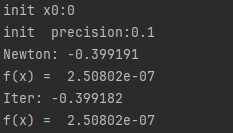
\includegraphics[width=12cm, height=6cm]{img/lab2_1_res.png}
\caption{Вывод программы в консоли}
\end{figure}
\pagebreak

\subsection{Исходный код}

\lstinputlisting{include/lab2_1/main.cpp}
\lstinputlisting{include/lab2_1/iter.cpp}
\lstinputlisting{include/lab2_1/iter.h}
\lstinputlisting{include/lab2_1/newton.cpp}
\lstinputlisting{include/lab2_1/newton.h}



\pagebreak

\section* {2.2  Методы простой итерации и Ньютона}

\subsection{Постановка задачи}
Реализовать методы простой итерации и Ньютона решения систем нелинейных уравнений в виде программного кода, задавая в качестве входных данных точность вычислений. С использованием разработанного программного обеспечения решить систему нелинейных уравнений (при наличии нескольких решений найти то из них, в котором значения неизвестных являются положительными); начальное приближение определить графически. Проанализировать зависимость погрешности вычислений от количества итераций. 

{\bfseries Вариант:} 24

\begin{cases}
& 3x^2_1 - x_1 + x^2_2 - 1 = 0 \\
&  x_2 - tg(x_1) = 0  \\
\end{cases}
%\pagebreak

\subsection{Результаты работы}
\begin{figure}[h!]
\centering
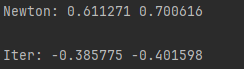
\includegraphics[width=15cm, height=6cm]{img/lab2_2_res.png}
\caption{Вывод программы в консоли}
\end{figure}
\pagebreak


\subsection{Исходный код}

\lstinputlisting{include/lab2_2/main.cpp}
\lstinputlisting{include/lab2_2/iter.cpp}
\lstinputlisting{include/lab2_2/iter.h}
\lstinputlisting{include/lab2_2/newton.cpp}
\lstinputlisting{include/lab2_2/newton.h}
